\documentclass[11pt]{article}
% amsmath package, useful for mathematical formulas
\usepackage{amsmath}
%\usepackage{natbib}
% amssymb package, useful for mathematical symbols
\usepackage{amssymb}
\usepackage{booktabs}
\usepackage{xspace}
% graphicx package, useful for including eps and pdf graphics
% include graphics with the command \includegraphics
\usepackage{graphicx}


% cite package, to clean up citations in the main text. Do not remove.
\usepackage{cite}
\usepackage{caption}
\usepackage{subcaption}

\usepackage{color} 

% Use doublespacing - comment out for single spacing
%\usepackage{setspace} 
%\doublespacing


% Text layout
\topmargin 0.0cm
\oddsidemargin 0.5cm
\evensidemargin 0.5cm
\textwidth 16cm 
\textheight 21cm

% Bold the 'Figure #' in the caption and separate it with a period
% Captions will be left justified
\usepackage[labelfont=bf,labelsep=period,justification=raggedright]{caption}

% Use the PLoS provided bibtex style
\bibliographystyle{/Users/stephens/Dropbox/Documents/stylefiles/plos2009}

% Remove brackets from numbering in List of References
\makeatletter
\renewcommand{\@biblabel}[1]{\quad#1.}
\makeatother


% Leave date blank
\date{}

\pagestyle{myheadings}
%% ** EDIT HERE **
\usepackage{enumerate}
\usepackage{multirow} 
\usepackage{url}
\usepackage{xr} %for cross-referencing
%% ** EDIT HERE **
%% PLEASE INCLUDE ALL MACROS BELOW
\newtheorem{algorithm}{Algorithm}
\newtheorem{proposition}{Proposition}
\newtheorem{restateproposition}{Proposition}
\newtheorem{lemma}{Lemma}
\newtheorem{corollary}{Corollary}
\newtheorem{result}{Result}
\newtheorem{note}{Note}
\newtheorem{definition}{Definition}

\begin{document}

\section{Pros and Cons of Admixture}

We talk about possible advantages and disadvantages that the admixture model or the topic model has over other methods like PCA, t-SNE or Hierarchical clustering. 

\subsection{Pros of admixture}

\begin{itemize}

\item The Structure plot is visually easy to interpret, specially when there is an ordering among the samples and there is a continuity in the cluster patterns related to the ordering. The best example is seen in the 2010 paper by Behar et al  (Figure 1)

\begin{figure*}[ht]
	\centering
	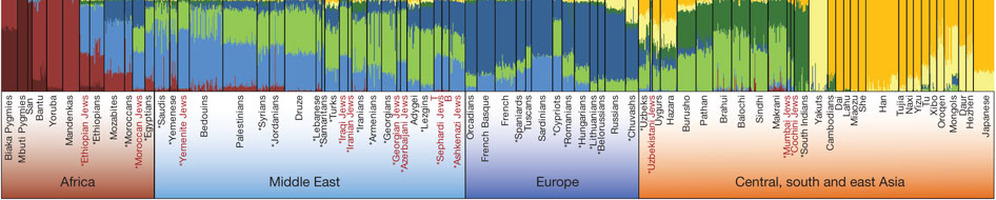
\includegraphics[height=2.5in, width=5in]{structure_continuity.png}
        \caption{Structure plot in population genetics study of Jewish people using genotype data. The mixing proportions represents the proportion of admixture in modern populations grouped by continents.}
\end{figure*}

We also saw a similar pattern in a single cell RNA-seq data from different parts of the renal tubule (Figure 2).

\begin{figure*}[ht]
	\centering
	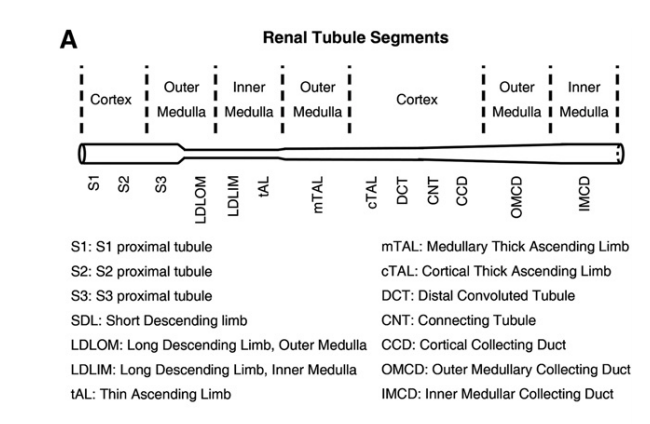
\includegraphics[height=2in, width=4in]{renal_tubule.png}
        \caption{Renal tubule segments}
\end{figure*}

The Structure plot of the cells from different parts of the renal tubule (Figure 3).

\begin{figure*}[ht]
	\centering
	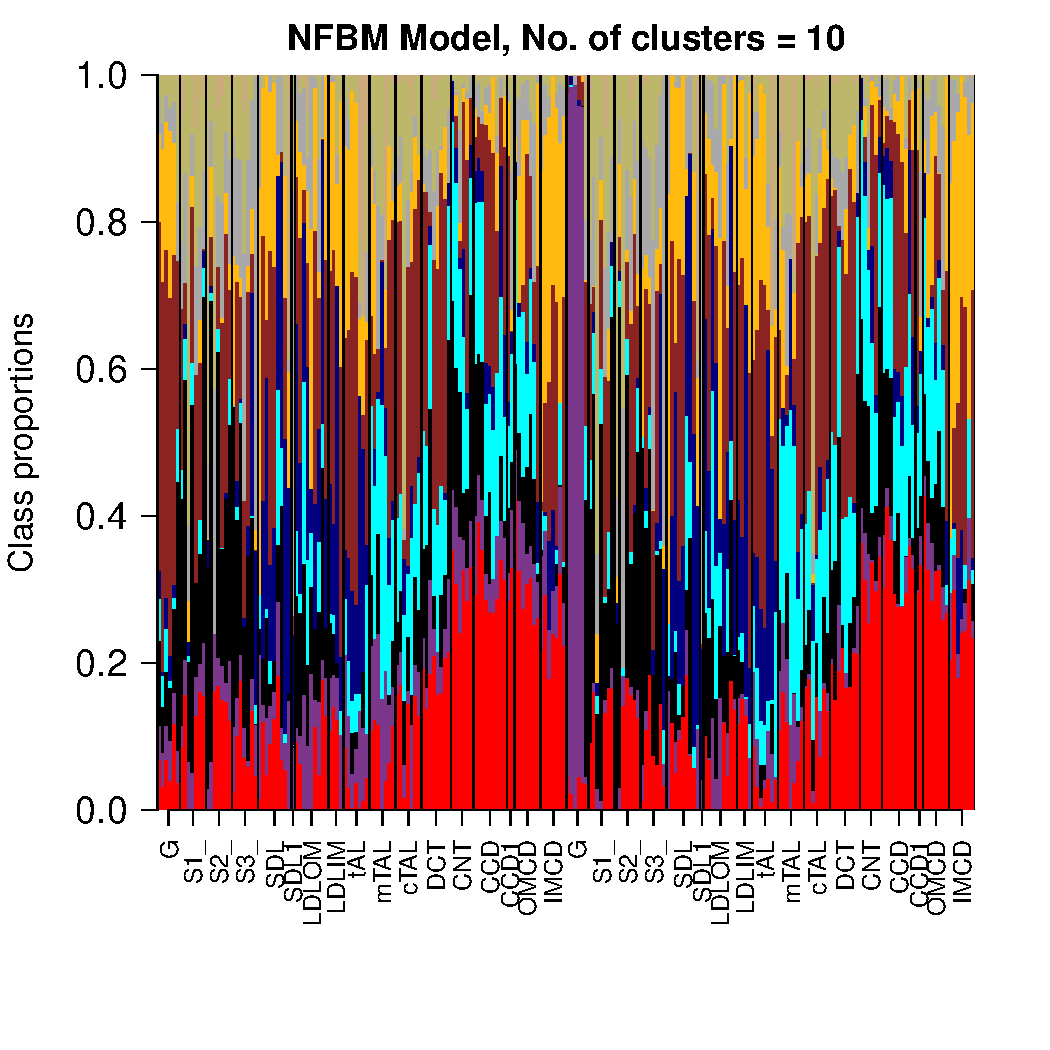
\includegraphics[height=2.5in, width=6in]{Structure_model_batch_nephron.pdf}
        \caption{Structure plot of the renal tubule data}
\end{figure*}

This continuity feature is pretty much exclusive to the Structure plot and is not reflected by PCa or tSNE or hierarchical clustering.

\item Sometimes the interest lies in figuring out the transition point from one cluster to another and which samples represent the transition point and what are the metadata underlying those samples that could be important information.  Structure plot highlights those transition points way better than PCA or t-SNE (Figure 4).

\begin{figure*}[ht]
	\centering
	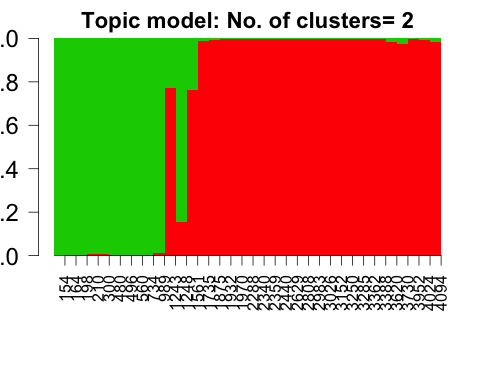
\includegraphics[height=2.5in, width=4in]{elevation_clustering.png}
        \caption{The Structure plot of the Himalayan forest spots based on bird abundance data with the columns representing forest spots at different elevations, the spots being arranged as per elevation. The transition from one cluster to another seems to be occurring at  1300 m approx from sea level}
\end{figure*}

Such a thing is difficult to figure out from PCA or t-SNE. PCA performs still better for such a data in figuring out the clusters although the transition point is difficult to obtain (Figure 5 and Figure 6). 

\begin{figure*}[ht]
	\centering
	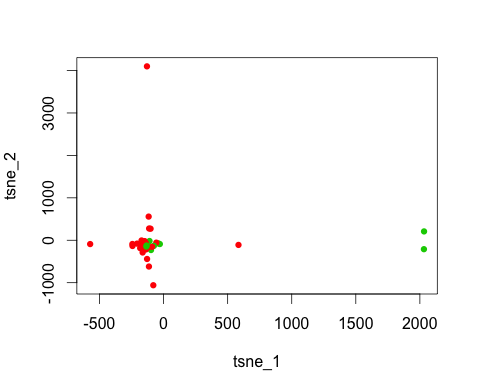
\includegraphics[height=2.5in, width=4in]{tsne_plot.png}
        \caption{t-SNE plot of the forest spots.}
\end{figure*}

\begin{figure*}[ht]
	\centering
	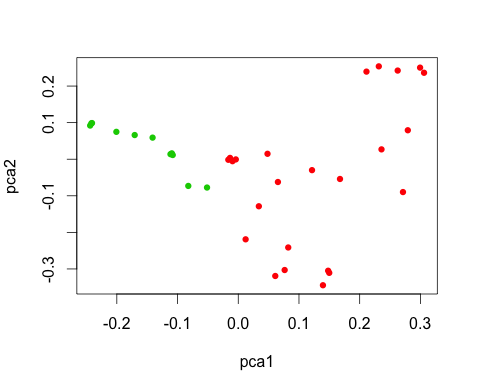
\includegraphics[height=2.5in, width=4in]{pca_plot.png}
        \caption{PCA plot of the forest spots (cluster colors obtained from admixture).}
\end{figure*}

\item Structure does a better job in clustering for counts data, specially cases where there are pretty small. As you saw from the above analysis, t-SNE failed badly and even for PCA, if we did not know the cluster labels from the admixture plot, then it would have been difficult to figure out the clustering partition as it is not clear (Figure 7). 

\begin{figure*}[ht]
	\centering
	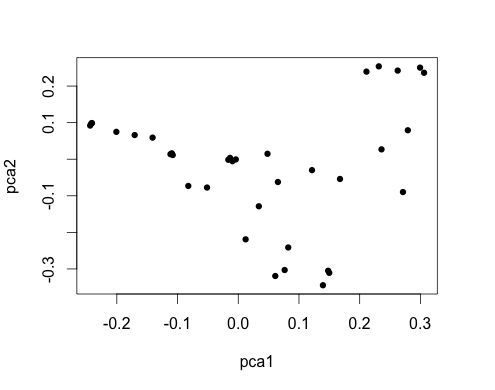
\includegraphics[height=2.5in, width=4in]{pca_plot_2.png}
        \caption{PCA plot of the forest spots.}
\end{figure*}

Also when there are two groups in the dataset but they are pretty close, then Structure outperforms hierarchical clustering (figure in the RNA-seq paper). 

\item The topic model gives us a model loglikelihood or Bayes factor for different choices of number of clusters $K$. This helps us determining the optimal number of clusters and also since it is model based, it has predictive strength. If a new sample is coming in with its own set of counts, then we can predict the admixture proportions corresponding to different groups for that sample as well. Usual methods like hierarchical clustering, PCA or tSNE do not have this power.

\end{itemize}

\subsection{Cons of admixture}

\begin{itemize}

\item The method can only be applied on counts data whereas PCA, tSNE or hierarchical clustering are general clustering tools.

\item Over dispersion  (mainly originating in cases of very large counts as well as very small counts) can bias the results.

\item It has been observed through simulation studies that the topic proportions may not always be a reliable estimate of the actual admixture proportion of underlying subgroups. However, the list of driving OTUs or genes that drive the clusters remains preserved or is robust even when admixture proportions are off. 

\end{itemize}
\end{document}




